\chapter{Mathematical Preliminaries}
\label{chapter:mathematical-preliminaries}

This chapter is intended to serve as a reference point for the more fundamental concepts that are used throughout this dissertation. In particular, this dissertation contains a significant amount of  discussion on \textit{Formal Concept Analysis} and \textit{Preference Relations}; which, in turn, are based on order theory, which is where we begin. The second half of this chapter provides an introduction to basic notions in logic, given in the setting of propositional logic.

\section{Order and Lattice Theory}
\label{section:order-theory}

\subsection{Orders}
\label{subsection:orders}

\begin{definition}
  \label{definition:binary-relation}
  A \textbf{binary relation} \index{binary relation} $R$ over two sets $X$ and $Y$ is a set of ordered pairs $\langle x,y \rangle$ with $x \in X$ and $y \in Y$; and so $R \subseteq X \times Y$. In many cases we express this pair using infix notation, and we write $xRy$.
\end{definition}

Binary relations are not particularly interesting until they satisfy certain properties. We now discuss certain binary relations which occur frequently enough to deserve a distinct name.

\begin{definition}
  \label{definition:partial-order}
  A \textbf{partial-order} \index{partial-order} is a binary relation $\preceq \; \subseteq X \times X$ that satisfies the following properties:
  \begin{align}
    & \text{(Reflexivity)} & x \preceq x \\
    & \text{(Antisymmetry)} & x \preceq y \text{ and } y \preceq x \text{ implies } x = y \\
    & \text{(Transitivity)} & x \preceq y \text{ and } y \preceq z \text{ implies } x \preceq z
  \end{align}
  for all $x,y,z \in X$.
\end{definition}

We write $x \npreceq y$ to indicate that $x \preceq y$ does not hold, and $x \prec y$ for the case where $x\preceq y$ and $x \not = y$. When $x \not \preceq y$ and $y \not \preceq x$---i.e., that $x$ and $y$ are incomparable---we write $x \Vert y$ \cite{Davey_Priestley_2002}. From a partial-order we can quite easily induce the notion of a \emph{strict partial-order}.

\begin{definition}
  \label{definition:strict-partial-order}
  A \textbf{strict partial-order} \index{strict partial-order} is a binary relation $\prec \; \subseteq X \times X$ that satisfies:
  \begin{align}
    & \text{(Irreflexivity)} & x \nprec x \\
    & \text{(Asymmetry)} & x \prec y \text{ implies } y \nprec x \\
    & \text{(Transitivity)} & x \prec y \text{ and } y \prec z \text{ implies } x \prec z
  \end{align}
  for all $x,y,z \in X$.
\end{definition}

An ordered set is a pair $(X, \preceq)$ with $X$ being a set and $\preceq$ being an ordering on $X$. If $\preceq$ is a partial-ordering, we might then refer to $X$ as a \textit{poset}. We can describe ordered sets diagrammatically through the use of \textit{Hasse} diagrams\index{Hasse diagrams}.

\begin{figure}[H]
  \centering
  \begin{subfigure}{0.3\textwidth}
    \centering
    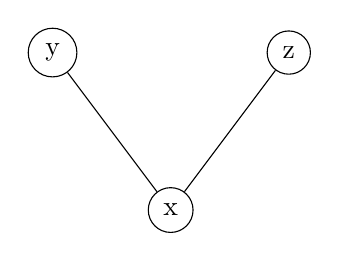
\begin{tikzpicture}[every node/.style={circle, draw, minimum size=0.25cm}]
      \node (y) at (-1.5,0) {y};
      \node (z) at (1.5,0) {z};
      \node (x) at (0,-2) {x};

      \draw (y) -- (x);
      \draw (z) -- (x);
    \end{tikzpicture}
    \subcaption{$\preceq_a$}
    \label{subfigure:partial-order-a}
  \end{subfigure}%
  \begin{subfigure}{0.3\textwidth}
    \centering
    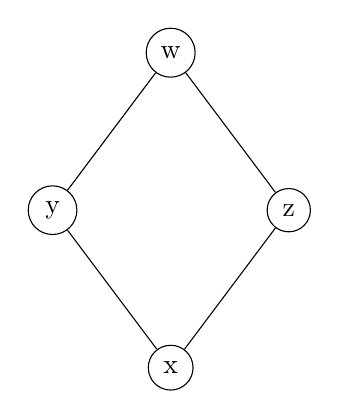
\begin{tikzpicture}[every node/.style={circle, draw, minimum size=0.25cm}]
      \node (w) at (0,2) {w};
      \node (y) at (-1.5,0) {y};
      \node (z) at (1.5,0) {z};
      \node (x) at (0,-2) {x};

      \draw (w) -- (y);
      \draw (w) -- (z);
      \draw (y) -- (x);
      \draw (z) -- (x);
    \end{tikzpicture}
    \subcaption{$\preceq_b$}
    \label{subfigure:partial-order-b}
  \end{subfigure}%
  \begin{subfigure}{0.3\textwidth}
    \centering
    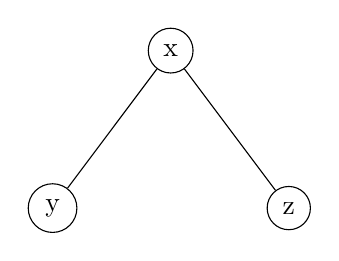
\begin{tikzpicture}[every node/.style={circle, draw, minimum size=0.25cm}]
      \node (y) at (-1.5,0) {y};
      \node (z) at (1.5,0) {z};
      \node (x) at (0,2) {x};

      \draw (y) -- (x);
      \draw (z) -- (x);
    \end{tikzpicture}
    \subcaption{$\preceq_a$}
    \label{subfigure:partial-order-c}
  \end{subfigure}%
  \caption{Three partial-orders over a set $P$}
  \label{figure:hasse-diagram}
\end{figure}

Then, a pair $\langle x,y \rangle$ is in a given binary relation $\preceq \; \subseteq X \times X$ if there exists a strictly upward path connecting $x$ to $y$ (or, if $x = y$). From \Cref{subfigure:partial-order-b} we can infer that $x \preceq_b y$, $x \preceq_b w$, and $y \Vert_b z$. For the inverse of an order $\preceq$ we write $\preceq^{-1}$, and so in \Cref{figure:hasse-diagram} $\preceq_a^{-1} = \preceq_c$ \cite{ganter1999formal}.

If $(X,\preceq)$ is an ordered set, then an element $x \in X$ is \textit{minimal} in $X$ if there exists no distinct element $y \in X$ such that $y \preceq x$. Conversely, $x$ is \textit{maximal} in $X$ if there exists no distinct $y \in X$ with $x \preceq y$. Continuing this example, $x$ is the \textit{minimum} of $X$ if it is minimal in $X$ and there are no elements to which $x$ is incomparable. In other words, for every element $y \in X$ it is the case that $x \preceq y$. Naturally, $x$ is the \textit{maximum} element of $X$ if for all $y \in X$ it is the case that $y \preceq x$.

\begin{definition}
  \label{definition:infimum-supremum}
  Let $(X,\preceq)$ be a partially ordered set, and $Y$ a subset of $X$. The \textbf{lower bound} of $Y$ is an element $x \in X$ with $x \preceq y$ for all $y \in Y$. The \textbf{upper bound} of $Y$ is defined dually. If the set of lower bounds of $Y$ has a maximum (greatest) element then this element is called the \textbf{infimum} of $Y$. Dually, if there is a minimum (least) element in the set of upper bounds, then this element is the \textbf{supremum} of $Y$.
  \index{supremum} \index{infimum}
\end{definition}

\subsection{Lattices}
\label{subsection:lattices}

\index{lattices}
Certain, particularly interesting, posets satisfy some nice properties involving infimums and supremums. Frequently, we call the supremum of elements $A = \{x,y,z\}$ of a poset the \textit{join}, and write $x \vee y$, or $\bigvee A$. The dual notion of an infimum corresponds to the \textit{meet}, and is written $x \wedge y$ or $\bigwedge A$.

\begin{definition}
  \label{definition:complete-lattice}
  A partially ordered set $\mathbf{X} = (X, \preceq)$ is a \textbf{lattice} if and only if, for any two elements $x, y \in \mathbf{X}$, both the supremum $x \vee y$ and the infimum $x \wedge y$ exist. The set $\mathbf{X}$ is a \textbf{complete lattice} if and only if the meet and join exist for every subset of $\mathbf{X}$.
\end{definition}

In \Cref{figure:hasse-diagram} only (b) is a lattice (and a complete lattice too). In fact, every finite lattice is a complete lattice \cite{ganter1999formal}.